\chapter{Telescope time and its value}\label{sec:usage}
The observation portal records, for every proposal, semester and instrument class, the time allocated and the
time charged; charged time includes slews, acquisition and readout. Figure~\ref{fig:time} and
Table~\ref{tab:projects} summarise it, Fig.~\ref{fig:cost} gives the cumulative cost, and Appendix~\ref{sec:semesters} gives every semester.

\begin{figure}[h]
\centering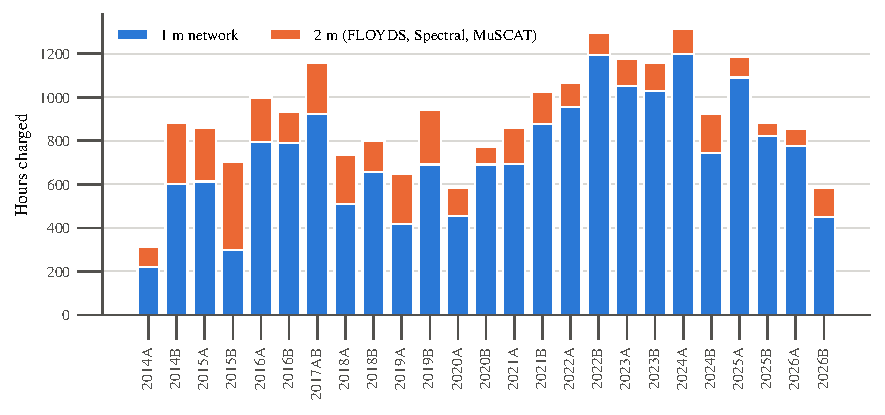
\includegraphics[width=\textwidth]{figures/fig_time_semester.pdf}
\caption{Telescope time charged per semester to the key projects, by telescope class. In 2014--2018 the 2-m time
is recorded as Spectral-camera time and includes the FLOYDS time.}\label{fig:time}
\end{figure}

\begin{table}[h]
\centering\small
\caption{Time charged and its value at current LCO prices, in pounds with dollars in parentheses
(\pounds\gbpOneM\,h$^{-1}$ = \$\usdOneM\,h$^{-1}$ on the 1-m network; 2-m time is not sold and is valued at \pounds\gbpTwoM\,h$^{-1}$ = \$\usdTwoM\,h$^{-1}$; \pounds\gbpPerUsd{} per \$). Images: reduced exposures in the
photometry database; spectra: FLOYDS science spectra.}\label{tab:projects}
\begin{tabular}{llrrrrrrr}
\toprule
Proposal & Semesters & 1-m (h) & 2-m (h) & Ms & \pounds\,M & (\$\,M) & Images & Spectra \\
\midrule
\inputtable{tables/tab_projects.tex}
\bottomrule
\end{tabular}
\end{table}

\begin{figure}[h]
\centering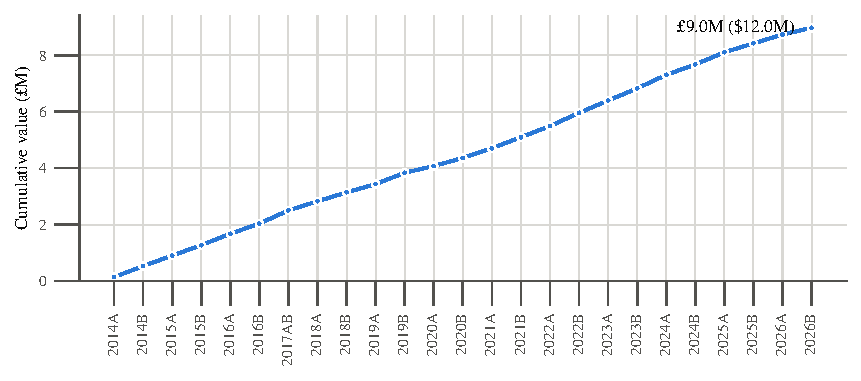
\includegraphics[width=\textwidth]{figures/fig_cost_cumulative.pdf}
\caption{Cumulative value of the time used, at current LCO prices (\pounds\gbpOneM\,h$^{-1}$ = \$\usdOneM\,h$^{-1}$ for
1-m time, an assumed \pounds\gbpTwoM\,h$^{-1}$ = \$\usdTwoM\,h$^{-1}$ for 2-m time).}\label{fig:cost}
\end{figure}

\paragraph{Value.} At the LCO price for 100\,h or more per year on the 1-m network (\pounds\gbpOneM\,h$^{-1}$,
\$\usdOneM\,h$^{-1}$) and an assumed \pounds\gbpTwoM\,h$^{-1}$ (\$\usdTwoM\,h$^{-1}$) for the 2-m telescopes, the
\hoursTotal~h used are worth \pounds\gbpTotal\,M (\$\usdTotal\,M). Pricing the 2-m time like the 1-m gives
\pounds\gbpTotalLow\,M (\$\usdTotalLow\,M), and scaling it by mirror area \pounds\gbpTotalHigh\,M (\$\usdTotalHigh\,M). Current prices are applied to all semesters.

\paragraph{Efficiency.} The open-shutter time is \expImagesMs~Ms for the images and \expSpectraMs~Ms for the FLOYDS
science spectra, against \msTotal~Ms charged. The imaging is about 70\,\% efficient on the 1-m network;
FLOYDS spends roughly two thirds of its charged time on acquisition, arcs, lamp flats and readout.
